\documentclass[12pt]{article}
\usepackage[margin=1in]{geometry}
\usepackage{titlesec}
\usepackage{parskip}
\usepackage{listings}
\usepackage{xcolor}
\usepackage{hyperref}
\usepackage[T1]{fontenc}
\usepackage{pagecolor} % For dark mode
\usepackage{graphicx}  % For images
\usepackage{float}     % For [H] float option

% Dark theme colors
\definecolor{darkbg}{HTML}{121212}
\definecolor{lighttext}{HTML}{E6E6E6}
\definecolor{codegray}{HTML}{2D2D2D}
\definecolor{accent}{HTML}{8DA0B6}

% Set page and text colors
\pagecolor{darkbg}
\color{lighttext}

% Configure hyperref for dark background
\hypersetup{
    colorlinks=true,
    linkcolor=accent,
    filecolor=accent,
    urlcolor=accent,
    citecolor=accent,
}

% Title formatting
\titleformat{\section}{\centering\Large\bfseries\color{accent}}{\thesection}{1em}{}
\titleformat{\subsection}{\large\bfseries\color{accent}}{\thesubsection}{1em}{}

% Code listing style
\lstset{
    backgroundcolor=\color{codegray},
    basicstyle=\ttfamily\footnotesize\color{lighttext},
    frame=single,
    breaklines=true,
    postbreak=\mbox{\textcolor{accent}{$\hookrightarrow$}\space},
    rulecolor=\color{accent},
}

\title{Instagram OSINT through Search Engine Techniques}
\author{}
\date{}

\begin{document}

\maketitle

\section{Introduction}

Open Source Intelligence (OSINT) gathering represents a critical methodology in cybersecurity assessments, digital investigations, and social media analysis. Advanced search operator techniques, often called ``search engine hacking,'' serve as foundational approaches within this domain. This paper examines a specific method tailored for extracting information from Instagram, one of the world's largest social media platforms.

\section{The Technique: Search Operator Implementation}

This approach combines two primary search operators to filter results with high precision, using the pattern: \texttt{site:"instagram.com" intext:"target-identifier"}.

\begin{itemize}
    \item \texttt{site:} This operator restricts the search to a specific domain. Using \texttt{site:"instagram.com"} confines results exclusively to pages hosted on Instagram's infrastructure.
    \item \texttt{intext:} This operator searches for pages containing a specific word or phrase within their visible text content. The placeholder \texttt{"target-identifier"} represents the specific username, real name, or other identifier of investigative interest.
\end{itemize}

The efficacy of this methodology stems from the logical conjunction of these operators. It directs the search index to return only results from Instagram's domain that simultaneously contain the exact specified search phrase.

\section{Application and Use Cases}

This technique's primary value lies not in locating primary profile pages (readily found through simple search), but in uncovering \textbf{secondary references} to accounts within the Instagram ecosystem. Practical applications include:

\begin{itemize}
    \item \textbf{Discovering Tagged Content:} Identifying public posts, stories, or reels where the target account has been referenced by other users, which may not be prominently visible on their primary profile.
    \item \textbf{Locating Mentions:} Finding posts where the target's identifier appears in captions or comment sections, potentially revealing connections, interactions, and conversations not otherwise documented.
    \item \textbf{Unearthing Historical Data:} Search engine cached versions of pages can sometimes reveal content that has been edited or removed from the live platform.
\end{itemize}

\section{Limitations and Ethical Considerations}

The effectiveness of this technique is inherently constrained by several factors:

\begin{itemize}
    \item \textbf{Privacy Settings:} This method only retrieves information from public Instagram profiles and posts. Content from private accounts remains inaccessible to search engine indexing.
    \item \textbf{Indexing Latency:} Search indices operate with significant delay; fresh content may not appear in results immediately after publication.
    \item \textbf{Platform Restrictions:} Search engine crawling agreements and Instagram's \texttt{robots.txt} directives can change, potentially limiting the scope of indexed content.
\end{itemize}

\textbf{Ethical Imperative:} This technique must be employed exclusively for legitimate OSINT purposes including security research, penetration testing, or authorized investigations. Any use for harassment, stalking, or unauthorized data collection violates ethical standards and potentially legal statutes. Researchers must maintain compliance with all applicable laws and platform terms of service.

\section{Practical Example: Tracing Digital Footprints}

To demonstrate the effectiveness of this approach, I conducted a small test scenario. First, I began by asking a language model for a stereotypically ``American'' name, which provided me with an example identifier (Figure \ref{fig:gpt}).

\begin{figure}[H]
    \centering
    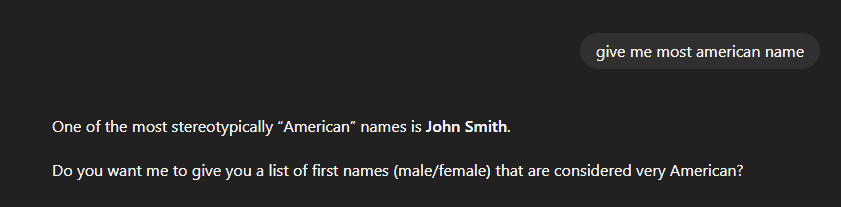
\includegraphics[width=0.6\linewidth]{1.png}
    \caption{Querying a language model for a stereotypically American name}
    \label{fig:gpt}
\end{figure}

Next, I located a private Instagram account registered with this identifier . While the account itself did not reveal any public photos, the username became the pivot point for further exploration.  

\begin{figure}[H]
    \centering
    
\includegraphics[width=0.6\linewidth]{2.png}
    \caption{Discovery of a private Instagram account}
    \label{fig:private}
\end{figure}

Applying the dork \texttt{site:"instagram.com" intext:"username"}, I was able to identify related mentions of the same handle across other Instagram pages (Figure \ref{fig:dork}).  

\begin{figure}[H]
    \centering
    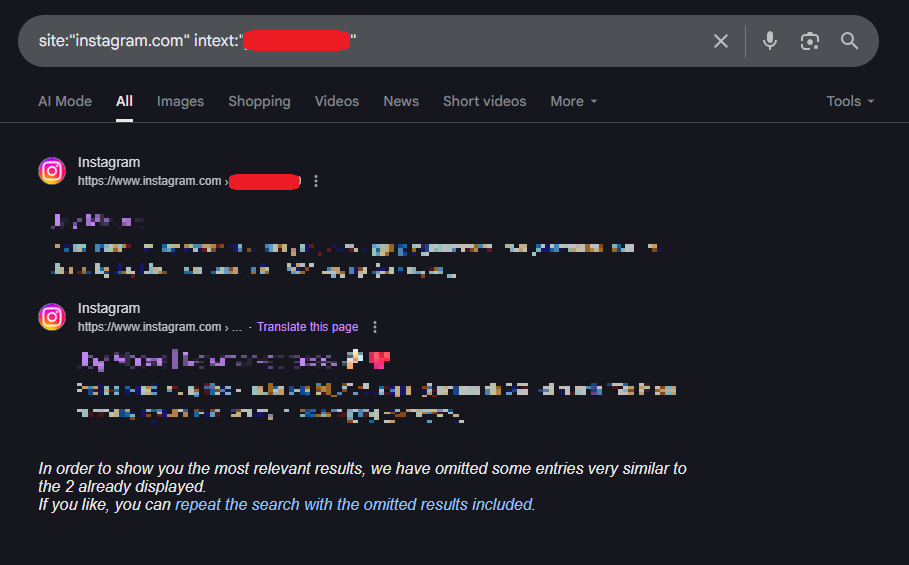
\includegraphics[width=0.7\linewidth]{3.png}
    \caption{Using Google dorking to locate related Instagram accounts}
    \label{fig:dork}
\end{figure}

Among these results was a connected friend’s account, which happened to be public. Unlike the private profile, this account exposed multiple images and interactions linked to the target (Figure \ref{fig:friend}).  

\begin{figure}[H]
    \centering
    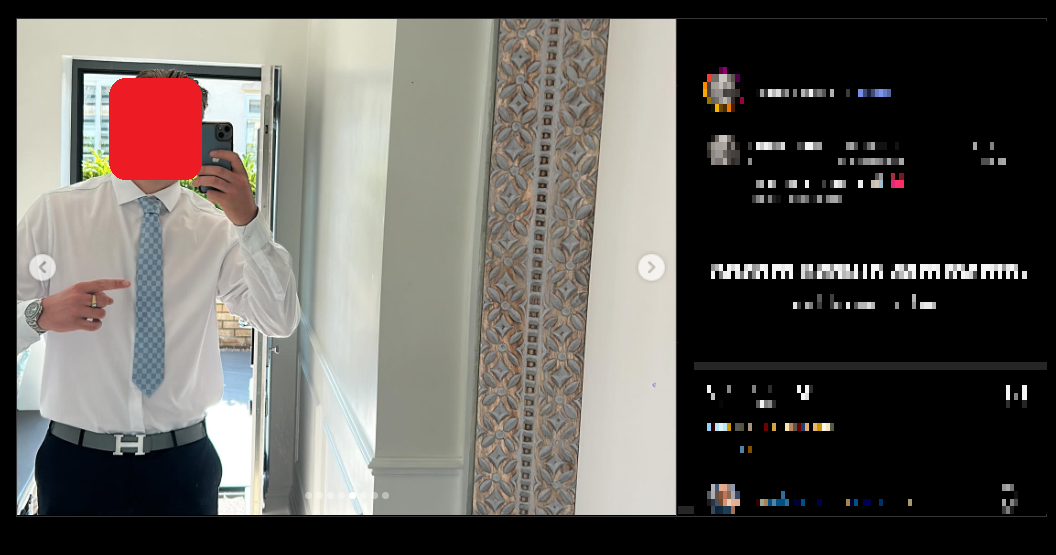
\includegraphics[width=0.6\linewidth]{4.png}
    \caption{Public friend’s account revealing multiple photos}
    \label{fig:friend}
\end{figure}

This illustrates how even when an account is private, secondary associations—friends, tags, or mentions—can leak publicly available content. The power of the dorking method lies in revealing these indirect digital footprints that a casual search would otherwise miss.

\clearpage
\listoffigures

\end{document}
